\subsection{Navigation Map}\label{subsec:navigation-map}

After the brainstorming session, the group started to create a navigation map~\cite{benyon2019}.
This map was made to visualize the flow of the user interface.
It features the different pages and how they are connected.
The navigation map can be seen in Figure~\ref{fig:navigation-map}.
Do note that the navigation map is representative of the final design and not the design of the prototypes.

The first page that the user interacts with is the login page.
From there they are directed to the dashboard, but they also have the choice to switch between the settings page and a
list of all the uploaded data.
The main focus for this project is the dashboard, where the user can see the different charts.
The settings page would allow the users to upload the data from their~\acrshort{epos} and to create categories for the
charts.
The total sales page shows a list of all the data without any visualization.
The user can also see visualization for a specific day from either the dashboard or the total sales page.

\begin{figure}[H]
    \centering
    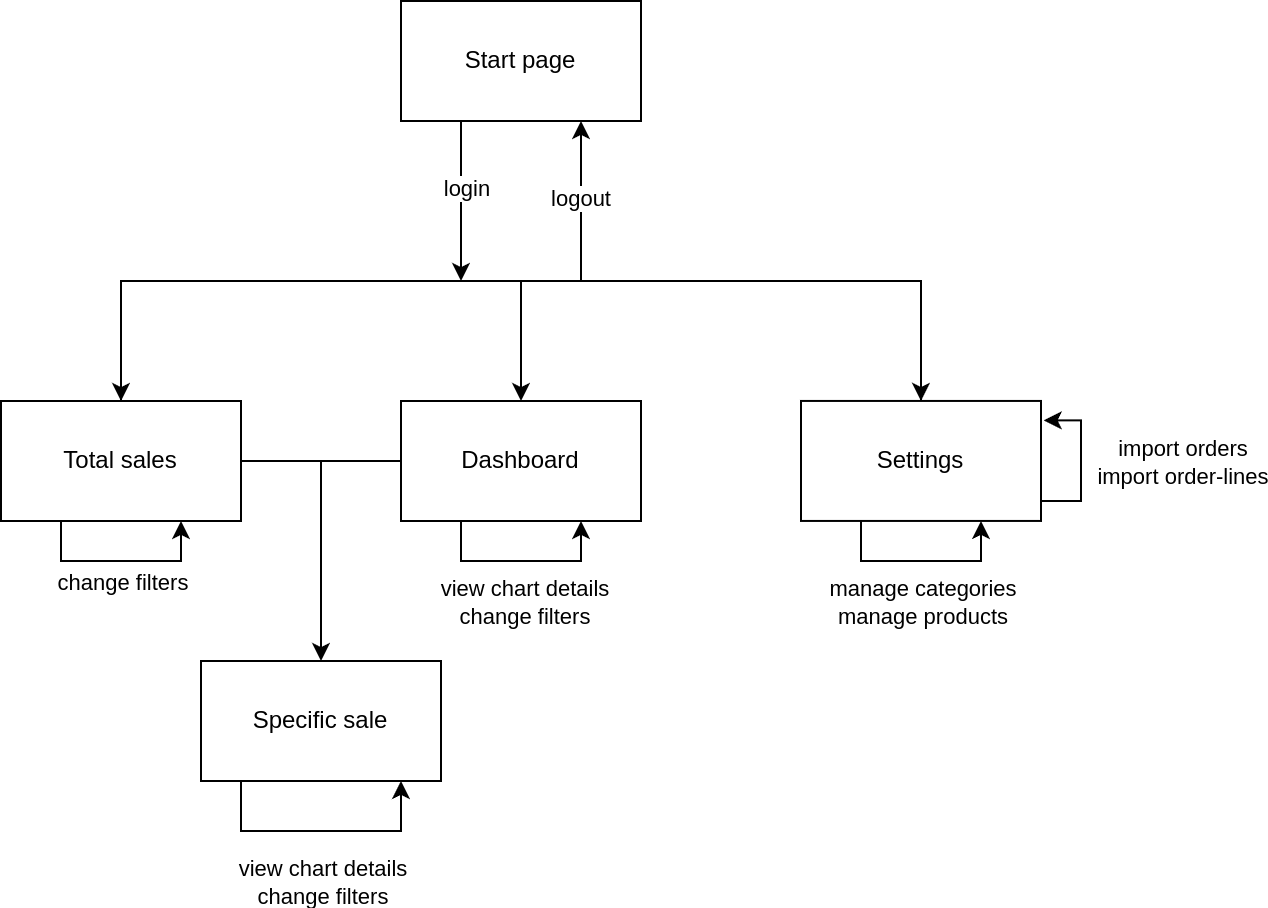
\includegraphics[width=\textwidth]{design-navigation-map.png}
    \caption{Navigation map of the final design.
    }\label{fig:navigation-map}
\end{figure}
